\documentclass[12pt]{article}
\usepackage{amsmath}
\usepackage{amssymb}
\usepackage{amsthm}
\usepackage{graphicx}
\usepackage{hyperref}
\usepackage{xcolor}
\usepackage{minted}
\usemintedstyle{vs}
\usepackage[latin1]{inputenc}
\usepackage[left=2.00cm, right=2.00cm, top=2.00cm, bottom=2.00cm]{geometry}
\newtheorem{theorem}{Theorem}[section]
\newtheorem*{problem}{Problem}
\newtheorem*{proposition}{Proposition}
\newtheorem*{corollary}{Corollary}
\newtheorem*{lemma}{Lemma}
\definecolor{light-gray}{gray}{0.95}
\title{\textbf{Running Hierarchical State Machines in Python with Asyncio}}
\author{}
\date{}
\begin{document}
\maketitle
This document describes the \texttt{async\_hsm} package for running Hierarchical State Machines (HSM) in Python using the single-threaded asyncio paradigm. The core algorithm is based on work by Miro Samek described in the book ``Practical UML Statecharts in C/C++'' and the code was forked from the \texttt{farc} project by Dean Hall.

Like a normal finite state machine (FSM), an HSM consists of states which are connected by transitions which are triggered by \emph{events}. The hierarchical aspect of HSMs allows states to be nested within one other in parent-child relationships. The machine is in only one state at a time. Each state may have an entry action and an exit action specified, which are performed when the state is entered or exited. Each state recognizes a set of events, and the arrival of such an event will cause an action to take place. The event may or may not specify a transition to a target state. If an event is not recognized by a state, the enclosing (ancestor) states in the hierarchy are examined until one is found that does handle the event. If the event does not specify a state transition, the action is performed and the machine remains in the \emph{original} (inner) state, even though the handler is defined in the outer state. On the other hand, if the event \emph{does} cause a transition to a target state, the action is performed
and all the exit actions associated with going from the original state to the outer state which handles the event are obeyed before making the transition to the target state. If all the ancestors of a state do not handle an event, it is silently handled by an implicit top state which is defined as the common ancestor of all the states. This causes no state transition, and so the event is effectively ignored. 

Performing a transition between two states in an HSM involves exiting states up to the last common ancestor (LCA) followed by entering states to the target state. All the exit and entry actions along the path are carried out. Note that we distinguish between remaining in the same state and transitioning from a state to itself. When transitioning from a state to itself, the exit action for the state is performed followed by the entry action. When remaining in a state, neither entry nor exit actions are performed. Following a transition to the target state, any initialization action defined for that state is performed, which will result in further state transitions.

When an HSM handles an event, the transitions and actions that it causes run to completion. In other words, any events that occur while the original event is being handled are just placed on an event queue,  whether they arise from external sources or are generated within the actions performed during the processing. The next event is not fetched from the event queue until after processing of the first event is complete.

\begin{figure}[h]
\centering
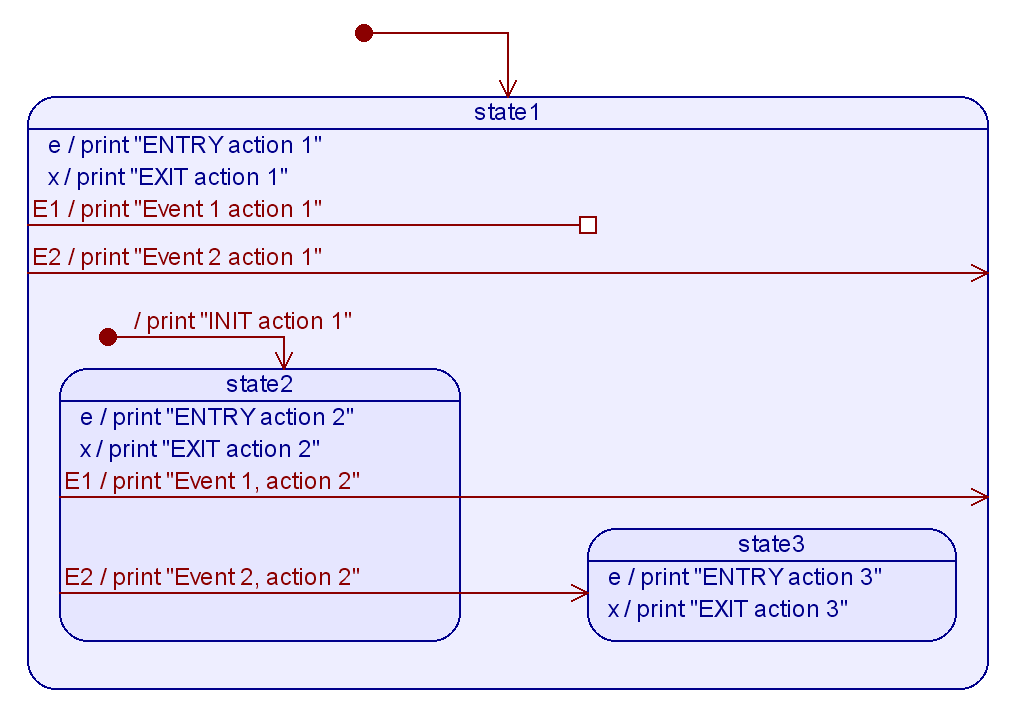
\includegraphics[width=0.7\linewidth]{SM_of_Example_1}
\caption[Example of state transitions in an HSM]{Example state transitions in an HSM}
\label{fig:smofexample1}
\end{figure}

Referring to Figure \ref{fig:smofexample1}, let us consider the behavior of the HSM in response to several events.
\begin{itemize}
	\item Since the initial state is defined to be \texttt{state1}, \texttt{ENTRY action 1} will be executed as the state is entered. Since \texttt{INIT action 1} is defined, this will be performed next, followed by a transition to \texttt{state2}, which causes execution of \texttt{ENTRY action 2}.
	
	\item Suppose that \texttt{EVENT1} is received. Since this is handled by \texttt{state2}, the action \texttt{EVENT1 action 2} is performed followed by a transition to \texttt{state1} which performs \texttt{EXIT action 2}. Note that we do \emph{not} exit \texttt{state1}. Since \texttt{INIT action 1} is defined, this will be performed next, followed by a transition to \texttt{state2}, which causes execution of \texttt{ENTRY action 2}.
	
	\item Next, suppose that \texttt{EVENT2} is received. Since this is handled by \texttt{state2}, the action \texttt{EVENT2 action 2} is performed followed by a transition to \texttt{state3} which performs \texttt{EXIT action 2} followed by \texttt{ENTRY action 3}.
	
	\item Next, suppose that \texttt{EVENT1} is received. Since this is not handled by \texttt{state3}, we examine the parent \texttt{state1} which does handle it. This involves performing \texttt{EVENT1 action 1} but \emph{no} state transition, which leaves the machine in \texttt{state3}.
	
	\item Finally, suppose that \texttt{EVENT2} is received. Since this is not handled by \texttt{state3}, we examine the parent \texttt{state1} which does handle it. The action \texttt{EVENT 2 action 1} is performed, which is followed by a transition, so we exit \texttt{state3}, performing \texttt{EXIT action 3} to get up to \texttt{state1}. We then perform the transition from \texttt{state1} to itself. As discussed previously, this causes \texttt{EXIT action 1} followed by \texttt{ENTER action 1} to be performed. Since \texttt{INIT action 1} is defined, this will be performed next, followed by a transition to \texttt{state2}, which causes execution of \texttt{ENTRY action 2}.
		
\end{itemize}

The event handling portion of an HSM is coded in the class \texttt{Hsm}. Instances of this class have a method called \texttt{dispatch} which takes an \texttt{Event} and performs all the actions and state transitions caused by that event before returning. The class \texttt{Ahsm} (an Augmented Hierarchical State Machine) is a subclass of \texttt{Hsm} which adds an event queue together with methods to post events to the queue using the FIFO or the LIFO discipline. In order to run a single HSM, it would be possible to write a task which fetches from the event queue and calls the \texttt{dispatch} method to process that event to completion before looping to fetch the next event. In the \texttt{async\_hsm} package, a separate \texttt{Framework} class is provided which allows a collection of inter-communicating \texttt{Ahsm} instances to be run concurrently. The operation of the \texttt{Framework} will be described in more detail later.

In normal use, an HSM is specified by subclassing \texttt{Ahsm}. Its operation is defined by writing ``state methods,'' one for each state of the machine. State transitions take place in response to namedtuples of type \texttt{Event}. Each such \texttt{event} has two parts, the first \texttt{event.signal} indicates the type of the event, while the second \texttt{event.value} can be any payload associated with the event. The type of an event is a \texttt{Signal}, which effectively acts as an enumeration. In order to create a signal named \texttt{SIGUSER}, the name is registered with the class by calling \texttt{Signal.register("SIGUSER")}. After performing this registration, we may use the notation \texttt{Signal.SIGUSER} and construct an event such as \texttt{Event(Signal.SIGUSER, payload)} which has \texttt{event.signal = Signal.SIGUSER} and \texttt{event.value = payload}.

The following code listing shows how the HSM in Figure 1 may be encoded as methods a class:

\begin{minted}
[
baselinestretch=1.0,
bgcolor=light-gray,
fontsize=\footnotesize,
linenos
]	
{python}
from async_hsm import Ahsm, Event, Signal, state

class HsmExample1(Ahsm):
    @state
    def _initial(self, event):
        Signal.register("E1")
        Signal.register("E2")
        return self.tran(self.state1)

    @state
    def state1(self, e):
        sig = e.signal
        if sig == Signal.ENTRY:
            print("ENTRY action 1")
            return self.handled(e)
        elif sig == Signal.EXIT:
            print("EXIT action 1")
            return self.handled(e)
        elif sig == Signal.INIT:
            print("INIT action 1")
            return self.tran(self.state2)
        elif sig == Signal.E1:
            print("Event 1 action 1")
            return self.handled(event)
        elif sig == Signal.E2:
            print("Event 2 action 1")
            return self.tran(self.state1)
        return self.super(self.top)

    @state
    def state2(self, e):
        sig = e.signal
        if sig == Signal.ENTRY:
            print("ENTRY action 2")
            return self.handled(e)
        elif sig == Signal.EXIT:
            print("EXIT action 2")
            return self.handled(e)
        elif sig == Signal.E1:
            print("Event 1 action 2")
            return self.tran(self.state1)
        elif sig == Signal.E2:
            print("Event 2 action 2")
            return self.tran(self.state3)
        return self.super(self.state1)


    @state
    def state3(self, e):
        sig = e.signal
        if sig == Signal.ENTRY:
            print("ENTRY action 3")
            return self.handled(e)
        elif sig == Signal.EXIT:
            print("EXIT action 3")
            return self.handled(e)
        return self.super(self.state1)
\end{minted}
Each state method is decorated using \texttt{@state}. A state function is invoked with an argument \texttt{e} which is the event that it needs to handle. As mentioned previously, \texttt{e.signal} is a signal defining the type of the event and \texttt{e.value} is the payload. Every state function must return one of the following, depending on the type of the signal

\begin{itemize}
	\item \texttt{self.handled(e)}. This indicates that the event has been handled and should not cause a state transition. Events of type \texttt{Signal.ENTRY} and \texttt{Signal.EXIT} should always return in this way if they are handled.
	
	\item \texttt{self.tran(next\_state)}. This indicates that the machine should transition to \texttt{next\_state} (which is a state method) when an event of this type occurs. An event of type \texttt{Signal.INIT} should return with a transition to a substate of the current state if it is handled.

	\item \texttt{self.super(parent\_state)}. This should be the default return value. The method gets here if the event is not explicitly handled within this state. Note that this default return value informs the code of the identity of the parent of this state. For states which do not have an explicit parent, the return value should be \texttt{self.super(self.top)} since \texttt{self.top} is an internally generated top level state which is the ancestor of all user-defined states.
\end{itemize}

In the listing, we see how each state method essentially goes through the possible signals in the event passed to it and handles each of them if it can. It should be evident how the code may be written down directly from the state chart of Figure \ref{fig:smofexample1}. The parent of each state is specified in the last return statement of the method, which is executed if the event is not explicitly handled otherwise.


Note that a special state method \texttt{\_initial} is required which is used to specify the transition to the actual initial state. This method is called once when the machine is entered, and so is also useful for performing any other initialization required, such as registering signal types.
 
\begin{minted}
[
baselinestretch=1.0,
bgcolor=light-gray,
fontsize=\footnotesize,
linenos
]	
{python}
async def main():
    hsm = HsmExample1()
    hsm.start(0)
    while not hsm.terminated:
        sig_name = input('\tEvent --> ')
        try:
            sig = getattr(Signal, sig_name)
        except LookupError:
            print("\nInvalid signal name", end="")
            continue
        event = Event(sig, None)
        hsm.dispatch(event)
    await Framework.done()

if __name__ == "__main__":
    asyncio.run(main())
\end{minted}

In order to run the hierarchical state machine, we may call its  \texttt{dispatch} method, passing in the event that we require it to handle. The above listing provides a simple interactive script which prompts the user for a signal to be handled by the HSM. The line \texttt{await Framework.done()} will be discussed in more detail later, it ensures that the \texttt{main} co-routine does not exit until all the state machines associated with the \texttt{Framework} have terminated. The output of the program is shown below for the sequence of events described in the example above.
\begin{minted}
[
baselinestretch=1.0,
bgcolor=light-gray,
fontsize=\footnotesize,
linenos
]
{text}
ENTRY action 1
INIT action 1
ENTRY action 2
        Event --> E1
Event 1 action 2
EXIT action 2
INIT action 1
ENTRY action 2
        Event --> E2
Event 2 action 2
EXIT action 2
ENTRY action 3
        Event --> E1
Event 1 action 1
        Event --> E2
Event 2 action 1
EXIT action 3
EXIT action 1
ENTRY action 1
INIT action 1
ENTRY action 2
        Event -->
\end{minted}
The state machine is run within a coroutine \texttt{main} using the \texttt{asyncio.run} function. In this simple example, a sequence of \texttt{Event} messages is sent to the state machine one-by-one using the \texttt{dispatch} method. More generally as a result of performing the actions associated with the state machine, new events may be generated. The methods \texttt{postFIFO} and \texttt{postLIFO} are defined on the \texttt{Ahsm} class and these allow events to be enqueued for processing after the current event handler has run to completion. 

The following code fragment shows how a sequence of events (specified in \texttt{seq} followed user-provided input) may be processed. Each event is placed on the queue (using \texttt{postFIFO}) and the \texttt{dispatch} method is called in a loop while the queue still has elements in it. In this way, events placed on the message queue during the running of the state machine are processed and run to completion before the next user event is enqueued.

\begin{minted}
[
baselinestretch=1.0,
bgcolor=light-gray,
fontsize=\footnotesize,
linenos
]	
{python}
async def main():
    hsm = HsmExample1()
    seq = ['E1', 'E2', 'E1', 'E2']
    hsm.start(0)
    while not hsm.terminated:
        if seq:
            sig_name = seq.pop(0)
            print(f'\tEvent --> {sig_name}')
        else:
            sig_name = input('\tEvent --> ')
        try:
            sig = getattr(Signal, sig_name)
            hsm.postFIFO(Event(sig, None))
        except LookupError:
            print("\nInvalid signal name", end="")
            continue
        while hsm.has_msgs():
            event = hsm.pop_msg()
            hsm.dispatch(event)
    print("\nTerminated")
    await Framework.done()

if __name__ == "__main__":
    asyncio.run(main())
\end{minted}
Running this program gives the same output as given above. At the prompt, additional events can be given or the \texttt{Ctrl-C} key combination may be entered. The latter generates an \texttt{Event.TERMINATE} message that is posted to the message FIFOs of the state machine(s). Within the internally-generated \texttt{top} state handler method, the \texttt{Event.TERMINATE} message causes a transition to the \texttt{\_exit} state. In this state, the \texttt{terminated} attribute of the machine is set, causing the program to break out of the loop. The last line of the \texttt{main} function \texttt{await Framework.done()} waits until all state machines in the framework have set their \texttt{terminated} attributes.

\begin{figure}[h]
\centering
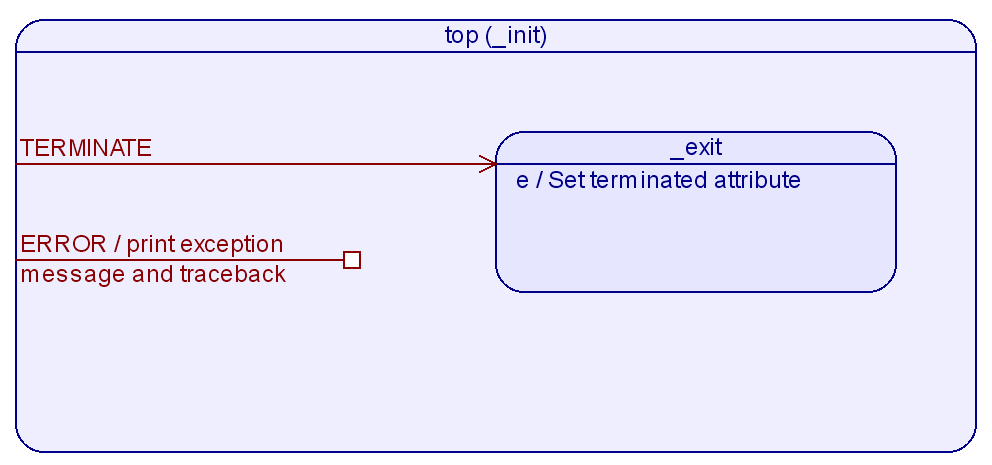
\includegraphics[width=0.7\linewidth]{internally_generated_states}
\caption[Internally generated HSM states]{Internally generated HSM states}
\label{fig:internallygeneratedstates}
\end{figure}

\subsection*{Error Handling}
If an exception is raised within any of the state-handler methods of an HSM class, the exception is caught and information about the exception is packaged into a special event whose signal type is \texttt{Signal.ERROR}. By default, this is posted to the message FIFO of state machine in which the exception was raised. The payload of the event (in its \texttt{value} attribute) is a dictionary with the following keys:
\begin{description}
\item[exc] The Python exception object
\item[traceback] A string with the traceback for the exception
\item[location] The name of the class in which the exception occurred
\end{description}
Within the internally-generated \texttt{top} state handler method, the \texttt{ERROR} event causes the exception message and traceback to be printed on the console, without a change of state.

In order to demonstrate how exceptions are handled by default, add the line \texttt{1/0} immediately following the line \texttt{print("Event 1 action 2")} in the state handler method \texttt{state2}. The result of the run changes to:

\begin{minted}
[
baselinestretch=1.0,
bgcolor=light-gray,
fontsize=\footnotesize,
linenos
]
{text}
ENTRY action 1
INIT action 1
ENTRY action 2
        Event --> E1
Event 1 action 2
Exception division by zero
Traceback (most recent call last):
  File "c:\github\async_hsm\async_hsm\__init__.py", line 382, in dispatch
    r = s(event)  # invoke state handler
  File "c:\github\async_hsm\async_hsm\__init__.py", line 155, in func_wrap
    result = func(self, evt)
  File "Hsm_example1.py", line 45, in state2
    1 / 0
ZeroDivisionError: division by zero

        Event --> E2
Event 2 action 2
EXIT action 2
ENTRY action 3
        Event --> E1
Event 1 action 1
        Event --> E2
Event 2 action 1
EXIT action 3
EXIT action 1
ENTRY action 1
INIT action 1
ENTRY action 2
        Event --> <Ctrl-C>
EXIT action 2
EXIT action 1

Invalid signal name
Terminated
\end{minted}
\section*{The Framework class for systems of hierarchical state machines}

When there is more than one hierarchical state machine, it is useful to have a framework within which all the machines can run. Each HSM is provided with its own event queue and is assigned a unique priority level. The framework is responsible for calling the dispatch function of each machine, passing it messages from its event queue. An HSM can post messages not only to its own queue, but can use the static method \texttt{publish} of the \texttt{Framework} class to post it to the queues of all machines which have opted to subscribe to messages of that type. In this way, machines can communicate with each other. The static method \texttt{Framework.subscribe} is passed a string with the name of the \texttt{Signal} to which the machine wishes to subscribe. 

It is important to define the sequence in which all the HSMs receive their messages. The framework starts with the machine with the highest priority and calls its dispatch method with the event (if any) at the head of its queue. It proceeds to the machine with the next highest priority and does the same, and continues until all machines have been handled. If any event queue is non-empty, the cycle repeats with the highest priority machine. New events can be placed on the event queue(s) from external sources such as timers, user input, or as a result of actions triggered by earlier events.

Using the static method \texttt{Framework.publish()} simplifies interacting with one or more state machines, since it sends the event to the state machines (which have subscribed) and then calls \texttt{Framework.run()} to perform all the actions that follow from that event. The following listing sends the sequence of events specified in \texttt{seq} to the state machine \texttt{HsmExample1}.

\begin{minted}
[
baselinestretch=1.0,
bgcolor=light-gray,
fontsize=\footnotesize,
linenos
]	
{python}
async def main():
    hsm = HsmExample1()
    seq = ['E1', 'E2', 'E1', 'E2']
    hsm.start(0)

    for sig_name in seq:
        sig = getattr(Signal, sig_name)
        print(f'\tEvent --> {sig_name}')
        Framework.publish(Event(sig, None))
        # Allow other tasks to run
        await asyncio.sleep(0)

    # Wait for CTRL-C to signal TERMINATE to all the HSMs
    await Framework.done()

if __name__ == "__main__":
    asyncio.run(main())
\end{minted}

It is necessary to subscribe to the events in the class \texttt{HsmExample1}. 
This can be done by modifying the \texttt{\_initial} method to use \texttt{Framework.subscribe} instead of \texttt{Signal.register} as shown. Note that it is also necessary to pass the state machine that wishes to subscribe to the signal as the second argument to \texttt{Framework.subscribe}.

\begin{minted}
[
baselinestretch=1.0,
bgcolor=light-gray,
fontsize=\footnotesize,
linenos
]	
{python}
    @state
    def _initial(self, event):
        Framework.subscribe("E1", self)
        Framework.subscribe("E2", self)
        return self.tran(self.state1)
\end{minted}


\end{document}


\section*{Running multiple state machines with additional asyncio tasks in an event loop}

When we need to run a collection of hierarchical state machines concurrently, the \texttt{asyncio} Python framework is used to manage their execution within a single event loop. 